\subsection{6. Матрицы смежности и инцидентности}

\subsubsection{6.1. Граф и его представления}

Пусть задан простой неориентированный граф $G = (V, E)$, где:
\begin{itemize}[leftmargin=*]
  \item $V = \{v_1, v_2, \dots, v_n\}$ — множество вершин ($|V| = n$),
  \item $E = \{e_1, e_2, \dots, e_m\}$ — множество рёбер ($|E| = m$).
\end{itemize}

Для хранения и анализа структуры графа удобно использовать его представление в виде матриц:
\begin{enumerate}[label=\arabic*)]
  \item \textbf{Матрица смежности} (adjacency matrix),
  \item \textbf{Матрица инцидентности} (incidence matrix).
\end{enumerate}

\subsubsection{6.2. Матрица смежности}

Матрица смежности $A$ — это квадратная матрица $n \times n$, где:
\[
  a_{ij} = \begin{cases}
    1, & \text{если вершины } v_i \text{ и } v_j \text{ соединены ребром}, \\
    0, & \text{иначе}.
  \end{cases}
\]

\textbf{Свойства:}
\begin{itemize}[leftmargin=*]
  \item Для неориентированного графа $A$ симметрична: $a_{ij} = a_{ji}$.
  \item Диагональные элементы $a_{ii}$ равны 1, если в графе есть петли (в простом графе всегда 0).
  \item Сумма элементов $i$‑й строки (или столбца) даёт степень вершины $v_i$.
\end{itemize}

\textbf{Пример:} граф с $V = \{v_1, v_2, v_3\}$ и рёбрами $E = \{(v_1,v_2), (v_2,v_3)\}$:

\[
A =
\begin{pmatrix}
  0 & 1 & 0 \\
  1 & 0 & 1 \\
  0 & 1 & 0 \\
\end{pmatrix}
\]

\subsubsection{6.3. Матрица инцидентности}

Матрица инцидентности $B$ — это матрица $n \times m$, где:
\[
  b_{ij} = \begin{cases}
    1, & \text{если вершина } v_i \text{ инцидентна ребру } e_j, \\
    0, & \text{иначе}.
  \end{cases}
\]

\textbf{Особенности:}
\begin{itemize}[leftmargin=*]
  \item Каждое ребро соединяет две вершины, значит в столбце $j$ ровно два значения 1 (если граф простой и без петель).
  \item В ориентированном графе обычно используют $-1$ и $+1$:  
    \[
    b_{ij} = \begin{cases}
      -1, & \text{если } v_i \text{ — начало дуги } e_j, \\
      +1, & \text{если } v_i \text{ — конец дуги } e_j, \\
      0, & \text{иначе}.
    \end{cases}
    \]
\end{itemize}

\textbf{Пример:} тот же граф, где $e_1 = (v_1,v_2)$, $e_2 = (v_2,v_3)$:

\[
B =
\begin{pmatrix}
  1 & 0 \\
  1 & 1 \\
  0 & 1 \\
\end{pmatrix}
\]

\subsubsection{6.4. Сравнение представлений}

\begin{itemize}[leftmargin=*]
  \item Матрица смежности подходит для быстрого ответа на вопрос: «Есть ли ребро между $v_i$ и $v_j$?»
  \item Матрица инцидентности удобна для анализа структуры рёбер, особенно в ориентированных графах.
  \item Для разреженных графов (мало рёбер) матрица смежности неэффективна по памяти.
\end{itemize}

\subsubsection{6.5. Визуальный пример}

\begin{center}
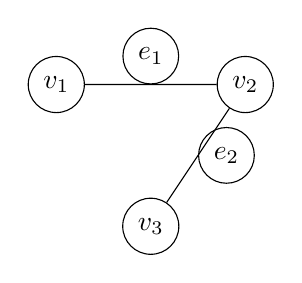
\begin{tikzpicture}[scale=1.2, every node/.style={circle, draw}]
  \node (v1) at (0,1.5) {$v_1$};
  \node (v2) at (2,1.5) {$v_2$};
  \node (v3) at (1,0)   {$v_3$};

  \draw (v1) -- (v2) node[midway, above] {$e_1$};
  \draw (v2) -- (v3) node[midway, right] {$e_2$};
\end{tikzpicture}

\vspace{0.5em}
\small Рис. 1. Граф с вершинами $v_1, v_2, v_3$ и рёбрами $e_1, e_2$
\end{center}

\subsubsection{6.6. Применения}

\begin{itemize}[leftmargin=*]
  \item Алгоритмы поиска в графе (например, обход в глубину, поиск кратчайших путей).
  \item Сетевые задачи (анализ маршрутов, потоков, связности).
  \item Работа с графами в программировании, машинном обучении и обработке изображений.
\end{itemize}

\subsubsection{Источники}

\begin{itemize}
  \item Гросс, Йелл: \emph{Теория графов и её приложения}.
  \item Д.Б. Уэст, \emph{Введение в теорию графов}.
  \item \href{https://ru.wikipedia.org/wiki/Матрица_смежности}{Википедия: Матрица смежности}
  \item \href{https://ru.wikipedia.org/wiki/Матрица_инцидентности}{Википедия: Матрица инцидентности}
\end{itemize}